\section{Projections}

To reinforce the idea that least squares problems are understood as projections, we'll take a projection problem and build the least squares problem from that.

%%
\subsection{Basic geometry}
Simplicity is under our control so we start with the $x-y$ plane and project a vector $b$ onto the plane. Using the vector
\begin{equation}
  b = \mat{c}{\frac{1}{2}\\\frac{1}{2}\\1}
\end{equation}
the projection onto the $x-y$ plane is simply
\begin{equation}
  \phi = \mat{c}{\frac{1}{2}\\\frac{1}{2}\\0}.
\end{equation}
Think of the projection as the ``shadow'' of the vector $b$. Figure \eqref{fig:lsq:proj} shows the geometry of this problem. The data vector projects out of the plane and is labelled as $b$. The shadow or orthogonal projection onto the plane is drawn in red and labeled as $\phi$. The dotted line shows that the vector $b$ is an orthogonal projection onto the plane.

\begin{figure}[htbp] %  figure placement: here, top, bottom, or page
   \centering
   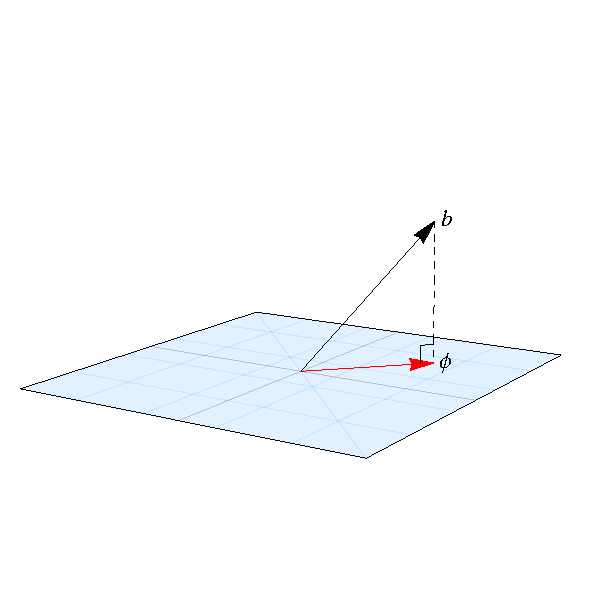
\includegraphics[ ]{pdf/lsq/linesp} 
   \caption{Projecting onto the plane. A vector $b$ projects out of the plane. The shadow of this vector in the plane is shown in red. This red vector $\phi$ marks the point in the plane which is closest to black vector. This closest point is the orthogonal projection of $b$ onto the plane.}
   \label{fig:lsq:proj}
\end{figure}

The crucial point is that the point $\phi$ is the closest point 
\textit{in the plane} to the point $b$. There are a few ways to visualize this notion of proximity. Image centering a tiny sphere at the point $b$. Allow the radius to increase until the sphere touches just one point in the plant. That point, the first contact, is $\phi$.

\begin{figure}[htbp] %  figure placement: here, top, bottom, or page
   \centering
   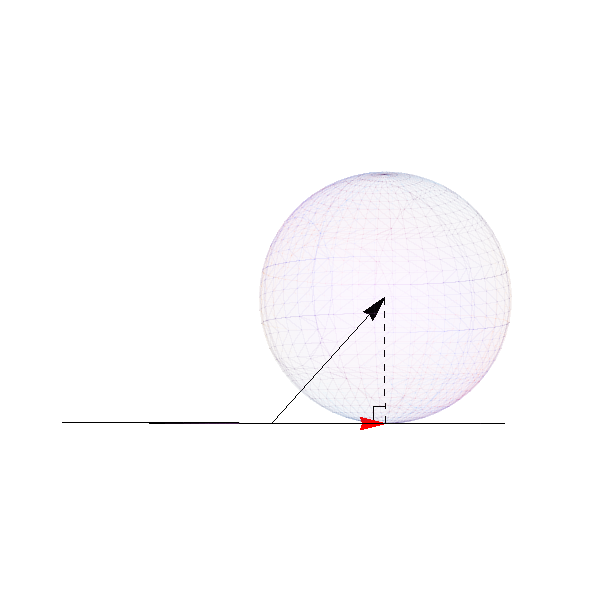
\includegraphics[ ]{pdf/lsq/sphere} 
   \caption{The osculating sphere. A sphere centered at the point $b$ grows until it first touches, or kisses, the plane. This point of osculation is the point in the plane closest to the center of the sphere.}
   \label{fig:lsq:sphere}
\end{figure}

The beauty of this geometric argument is that we are free of the notion of measurement. We don't need to measure the radius of the sphere; The point in the plane closest to the point $b$ lies along the radius of the sphere touching the plane at just one point.

%%
\subsection{Measuring distance}
Intuition is good, and additional seasoning with a dash of rigor can make the problem more enjoyable. Let's show that $\phi$ is the closest point in the plane. The strategy is simple: offset in the plane a finite distance to another point $\Phi$ and measure the distance from $\Phi$ to $b$, $d_{2}\paren{\Phi,b}$. This distance will necessarily be larger than the distance $d_{2}\paren{\phi,b}$. We are now forced to introduce a rule for measuring distance. The rule we choose is the familiar one of Pythagoras, also known as the 2$-$norm.

Call $\psi$ the vector in the plane which connects the projection $\phi$ to the offset point $\Phi$. The distance from $b$ to the plane is $b_{\perp}$. The distance from $\phi$ to $\Phi$ is $\psi$. The crucial distance is 
\begin{equation}
  d_{2}\paren{\Phi,b} = \normt{\psi+b_{\perp}} = \normt{\normt{\phi-\Phi}+b_{\perp}} = \paren{\phi-\Phi}^{2} + b_{\perp}^{2}.
\end{equation}
This distance is the smallest when $\phi = \Phi$; the distance is smallest when there is no offset from the point $\phi$. Therefore the point $\phi$ is the closest point in the plane to the point $b$. This smallest distance between the vector $b$ and its projection is given by
\begin{equation}
  d_{2} = \normt{b-\phi}=b_{\perp}.
\end{equation}

To finish the discussion, note that we used the 2$-$norm to measure distance. This was to make the discussion more concrete. The reality is that any $p-$norm would have worked.

%%
\subsection{Using the calculus}
An elementary method for finding the point in the plane closest to the vector is to minimize the distance between the point and the plane. It's easier to solve this problem in general. The distance between any vector and the plane is given by
\begin{equation}
  d_{2}\paren{b,\phi}=\normt{\mat{c}{x_{b}\\y_{b}\\z_{b}}-\mat{c}{x_{\phi}\\y_{\phi}\\0}} = \paren{\paren{x_{b}-x_{\phi}}^{2} + \paren{y_{b}-y_{\phi}}^{2} + z_{b}^{2}}^{1/2}.
\end{equation}
The closest point in the plane is 
\begin{equation}
  \phi = \mat{c}{x_{b}\\y_{b}\\0}
\end{equation}
and the separation is again
\begin{equation}
  d_{2}\paren{b,\phi} = z_{b}.
\end{equation}
The solution point minimizes the sum of the squares of the components of the vector connecting the vector to the plane.

%%
\subsection{The method of least squares - first formulation}
We have already solved this problem by minimizing the sum of the squares of distance between to points. Now let's formulate the problem for the method of least squares as 
\begin{equation}
 \A{}x=b.
\end{equation}
For this episode we will look for a solution vector
\begin{equation}
  x\in\cmplx{\by{2}{1}}
\end{equation}
which resticts the target matrix
\begin{equation}
  \A{}\in\cmplx{\by{ 3}{2}}_{2}.
\end{equation}

The $b$ vector is in hand, and what would be an appropriate matrix?

In this case the $x-y$ plane represents the \textit{image} of of the column vectors of the system matrix $\A{}$. We can pick any two vectors in the plane such as
\begin{equation}
  c_{1} = \mat{c}{1\\2\\0}, \quad c_{2} = \mat{r}{-1\\0\\0}
\end{equation}
and assemble the matrix as
\begin{equation}
  \A{} = \mat{c|c}{c_{1}&c_{2}}=\mat{r|r}{1&-1\\2&0\\0&0}.
\end{equation}
The linear system is given by
\begin{equation}
  \begin{array}{cccc}
    \A{} & x & = & b \\
    \mat{cr}{1&-1\\2&0\\0&0} & \mat{c}{x\\y} & = & \mat{c}{\frac{1}{2}\\\frac{1}{2}\\1}
  \end{array}
\end{equation}
and it only admits a least squares solution.

Of course we know how to recast this as a problem with a direct solution. We are confined to the range of the target matrix, $\rng{\A{}}$. This represents the closest formulation of the problem.
\begin{equation}
  \begin{array}{cccc}
    \A{} & x & = & \phi \\
    \mat{cr}{1&-1\\2&0\\0&0} & \mat{c}{x\\y} & = & \mat{c}{\frac{1}{2}\\\frac{1}{2}\\0}
  \end{array}
  \label{eq:lsq:form2}
\end{equation}
Using the knowledge of the orthogonal projection and the insight that least squares solutions are orthogonal projections we have traded a difficult problem for an elementary problem. The linear system can be solved by a reduction process. By inspection, the linear system in equation \eqref{eq:lsq:form2} can be written as
\begin{equation}
  \begin{split}
    x-y&=\frac{1}{2}.\\
    2x\qquad&=\frac{1}{2}.
  \end{split}
\end{equation}
The solution is
\begin{equation}
\boxed{
  x = \mat{c}{x\\y}=\frac{1}{4}\mat{r}{1\\-1}
  }.
\end{equation}

Notice the target matrix $\A{}$ cannot be inverted yet the linear system \eqref{eq:lsq:form2} can be solved.

Keep in mind that in a typical least squares problems the solution vector is not in a physical space with dimensions of measurements such as position or temperature. It is in a \textit{parameter space}. For example, with a least squares fit to a line (linear regression) where the model is
\begin{equation}
  y = m x + b
\end{equation}
the variables $x$ and $y$ are measurement locations and values; the solution vector is
\begin{equation}
  \mat{c}{slope\\intercept}=\mat{c}{m\\b}.
\end{equation}

%%
\subsection{The method of least squares - second formulation}
Consider the case where the solution
\begin{equation}
  x\in\cmplx{\by{3}{1}}
\end{equation}
and
\begin{equation}
  \A{}\in\cmplx{\by{3}{3}}_{2}.
\end{equation}

Typically when working on examples which depend on clear understanding of the domain and codomain it helps if the spaces have separate dimension. However, to maintain a sequence of examples we will consider a domain and codomain of equal dimension this single time.

To assemble the target matrix we choose three vectors from $\real{3}$. The first two vectors from the previous subsection can be recycled and we just need to add a new vector to write the problem as
\begin{equation}
  \begin{array}{cccc}
    \A{} & x & = & b, \\
    \mat{crc}{1&-1&1\\2&0&1\\0&0&0} & \mat{c}{x\\y\\z} & = &  \mat{c}{\frac{1}{2}\\\frac{1}{2}\\1}.
  \end{array}
  \label{eq:lsq:form3}
\end{equation}

Again we know that this least squares problem has the same solution as the system
\begin{equation}
  \begin{array}{cccc}
    \A{} & x & = & \phi, \\
    \mat{crc}{1&-1&1\\2&0&1\\0&0&0} & \mat{c}{x\\y\\z} & = & \mat{c}{\frac{1}{2}\\\frac{1}{2}\\0}.
  \end{array}
  \label{eq:lsq:form3}
\end{equation}
which has the direct solution via reduction
\begin{equation}
\boxed{
  x = \mat{c}{x\\y\\z}=\frac{1}{6}\mat{r}{1\\-1\\1}
  }.
\end{equation}

Again the target matrix $\A{}$ cannot be inverted, by the linear system {eq:lsq:form3} can be solved.

%%
\subsection{The method of least squares - third formulation}
Consider the case where the solution
\begin{equation}
  x\in\cmplx{\by{4}{1}}
\end{equation}
which implies
\begin{equation}
  \A{} \in \cmplx{\by{3}{4}}_{2}.
\end{equation}

We can just append another vector from $\real{3}$ to the previous target matrix:
\begin{equation}
  \begin{array}{cccc}
    \A{} & x & = & b, \\
    \mat{crcr}{1&-1&1&-1\\2&0&1&-1\\0&0&0&0} & \mat{c}{x\\y\\z\\t} & = &  \mat{c}{\frac{1}{2}\\\frac{1}{2}\\1}.
  \end{array}
  \label{eq:lsq:form4}
\end{equation}
This least squares problem has the same solution as the projected system
\begin{equation}
  \begin{array}{cccc}
    \A{} & x & = & \phi, \\
    \mat{crcr}{1&-1&1&-1\\2&0&1&-1\\0&0&0&0} & \mat{c}{x\\y\\z\\t} & = &  \mat{c}{\frac{1}{2}\\\frac{1}{2}\\0}.
  \end{array}
  \label{eq:system}
\end{equation}
 
Once more the linear system cannot be inverted, but it can be solved by elementary means. To wit, the two equations embodied in \eqref{eq:system} are these:
\begin{equation}
  \begin{array}{ccccccccc}
    2x&-&y&+&z&-&t&=&\frac{1}{2},\\
    x&&&+&z&-&t&=&\frac{1}{2}.\\
  \end{array}
\end{equation}
Subtracting bottom from top reveals that $x=-y$

\begin{equation}
\boxed{
  x = \mat{c}{x\\y\\z\\t}=\frac{1}{8}\mat{r}{1\\-1\\1\\-1}
  }\ .
\end{equation}
 
%%
\subsection{Relevance to the SVD}
We have solved a series of least squares problems without using the \svdl. What is the relevance to the SVD?
\begin{enumerate}
\item Greater insight into the geometry of the SVD solution;
\item Emphasize that the SVD solves the problem closest to
\begin{equation}
  \A{}x = b
\end{equation}
 
\end{enumerate}



\endinput